\documentclass[12pt]{report}
\usepackage{tikz}
\usepackage{cite}
\usepackage{listings}
\usepackage{url}
\usepackage{hyperref}
\RequirePackage{graphicx}
\graphicspath{ {images/} }
\newcommand{\ppt}{\textbf{p.p.t.}}
\newtheorem{theorem}{Theorem}[section]
\newcommand{\GF}{\text{GF}}
\newcommand{\xor}{\oplus}
\theoremstyle{definition}
\newtheorem{definition}{Def.}

\renewcommand{\collaborators}{Jiachun Zhang}

\begin{document}

\maketitle

\setcounter{MaxMatrixCols}{20} \setlength\parindent{0pt}

\section{Introduction}
The hearing of a music can be seen as a complex procedure of recognition. 
When we hear a piece of music, we can recognize the genre, characteristic, and 
style traits of its composer. Sometimes, we can immediately recognize
the similarity between two pieces of music, be it the reference from one to another
, same chord relation, or a signature musical device being used. In this project, 
we will make an attempt to examine the similarity between two pieces of music using 
various metrics ranging from the cosine similarity to DFT. The project will
survey on the existing methods of music similarity proposed by music theorists
Dimitri Tymoczko, David Lewin, and Jason Yust. As a related topic, the project has also
investigated the key-finding algorithm orginally proposed by Krumhansl and Schmuckler, 
modified by David Temperley. The final section of the report will be questions raised 
in the progress of reviewing these works and implementing the algorithms.

\section{Cosine Similarity}
Cosine similarity measures the cosine value of the angle between two vectors.
Given two melody, we can represent them as vectors of their pitch classes. (in set or
collection or ordered list) The angle decreases as the cosine value gets closer to 
1. The equation can be written as:
\[\cos(\theta) = \frac{\mathbf{A}\cdot\mathbf{B}}{|\mathbf{A}|\cdot|\mathbf{B}|}\]
where $\mathbf{A}$ and $\mathbf{B}$ are two vectors. The intuition behind this is that
the more notes in the melody are the same, the smaller the angle between the two vectors represented
by the melodies. The cosine similarity is a good measure of similarity between two melodies when it comes to
the overall "contour" of the melody. Given two melodies, one being Transposition of the other,
will still have the same cosine similarity. However, it does not measure anything harmonic wise
such as the scale the melody is in, or the chord progression implied when there are multiple voices
in the music. So we cannot simply put all the notes in the melody into a vector and calculate the cosine
distance between them.

\section*{Key Finding Algorithm}
\paragraph*{Krumhansl-Schmuckler Key Finding Algorithm}
The notion of key in tonal music can provide critical information of a music. Using the total duration
of each pitch class in a piece of music, we can calculate the probability of each key being the key of the
piece. We shall construct a profile of each pitch class in major and minor keys 
then find the corrilation coeficient between the profile and the pitch class distribution of the piece of music.
It measure the linear correlation between the profile value and the duraiton for each pitch class.
The key with the highest correlation is the key of the piece of music. The algorithm is as follows:
\[R(x,y)=\frac{\sum_i(x_i-\bar{x})(y_i-\bar{y})}{\sqrt{\sum_i(x_i-\bar{x})^2\sum_i(y_i-\bar{y})^2}}\]
where $x$ is the profile of the pitch class distribution of keys, and $y$ is 
the duration of each pitch class in the piece. Code can be found 
\href{https://github.com/StefanHeng/Symbolic-Music-Generation/blob/master/musicnlp/preprocess/key_finder.py}{here.}
Note, the code uses Temperley-Kosta-Payne profile here after trial and errors.
However, there are a few problems with this algorithm.
\begin{itemize}
    \item The notes are "weighted" by duration, which means repeated notes would take
    on more weight which might alter the final decision.
    \item It does not take into the account of modulation between different keys.
    \item The original key-profile model did not distinguish between different spelling fo
    the same pitch (A\#=Gb).
\end{itemize}
\paragraph*{Temperley Key Finding Algorithm}
David Temperley proposed a new key finding algorrithm to address these problems suing a 
Bayesian approach. The algorithm is as follows:
\[\arg \max_{\text{strcuture}}\Pr[\text{strcuture|surface}]\]. 
Since $\Pr[\text{surface}]$ stays the same, we only need to concider
$\Pr[\text{surface|strcuture}]\cdot\text{strcuture}$. To calculate 
the second term, we can design the following heuristics:
Start off with a probability of $\frac{1}{24}$ for every key. Then assign a 
very high probability to the same key meaning the composer will likely continue
compose in the key, but a low probability to any other key. Here Temperley uses
$0.8$ for the same key and $\frac{0.2}{24}$ for the rest. Bt intuitively, we want the rest
$0.2$ probability to be distributed according to likelyness of closely related key 
such as modulation or dominant. So a furhter discussion can be 
made on how to distribute the probability. As for the first term, Temperley porposed
a analyzing that first involves in segmentaiton of the piece:
\begin{enumerate}
    \item Partition the piece into segments of arbiturary length.
    \item Given a key-profile that contain probability of certain pitch class 
    played in the (major and minor) key, take the product of the present pitch 
    and the probability of the all absent pitch classes, which is 
    simply $1-$ the probability of its presence in the segment. Written as:
    \[\prod_p S(p)\prod_{\neg p}S(\neg p) \]
\end{enumerate}
Thus we get:
$\prod_m \Pr[\text{current key of segmen m}|\text{key of the last segment}]
\cdot\prod_p S(p)\prod_{\neg p}S(\neg p)$. We shall 
take the logarithm for a better numerical stability. The final equation is:
\[\sum_m (\ln\Pr[m|m']\sum_p\ln S(p)\sum_{\neg p}\ln S(\neg p))\]
A couple questions should be raised here:
\begin{itemize}
    \item How to determine the length of the segment?
    \item Should every notes in the segment be weighted equally?
\end{itemize}
Still, the algorithm discussed above is suitable only for a piece that is 
considered to have "one piece". Some times, the composer might trick the 
audience by writing multiple voices in different keys. For example
the left hand of Bartok's Bagatelles' No1 is in C Locrian, while the right hand is 
entrily in E Major. So we need to take into account of different voices as well. 

\section*{Similarity in terms of Voice Leading and Discrete Fourier Transform}
Like cosine similarity, we might want to talk about the similiarity between 
two set classes in terms of the difference between them, or the minimum movement
required for one to become the other, this is called voice leading. Dimitri Tymoszko
showed a new method of analyzing the voice leading distance using Discrete Fourier Transform.
The n-th Fourier component is (probably) inversly related to perfectly even
n note set class (chord). 
\paragraph*{Voice Leading Distance}
Between two n-note set classes $A$ and $B$, the minimal Euclidean voice leading 
distance can be founded as such:
\begin{enumerate}
    \item Find the prime form of $A$, the sum the its pitch classes is $m$.
    \item Find n transposition of B that sum up to $m$.
    \item For each transposition, find the minimal $l_2$ distance between 
    prome form of $A$ and circular permutations (permuation with same ordering)
    of transpositions. Do the same for all n inversions of B (?).
    \item The minimal distance within $2n^2$ numbers is the voice leading distance.
\end{enumerate}
\paragraph*{Discrete Fourier Transform}
The DFT of a set class can be written as:
\[\sum_p (\cos 2\pi pn/12, \sin 2\pi pn/12)\].
For $n\in \{1,2,3,4,5,6\}$, each nth Fourier component is the sum above.
The paper has showed, DFT converts the set class in a "reduced" circle with 
$12/n$ circumference. Each pitch in the set class is represented by a point
on the circle. The sum would be vector sum of all the points. If the pitch 
class lies closely to the set represneted by the perfectly even $n$-notes chord,
the vector will be close to the $0$ point. Thus the larger the magnitude of the
sum of the $n$-th Fourier component, the less movement is required in voice 
leading to the perfect $n$-note chord. Thus they form a inverse relationship.
Jason Yust , in his paper, gave another way of interpreting the DFT in terms of 
phase spaces and the vector in the phase spaces represented by pitch set class. Phase space $1$ to $6$
are all cicles with $12$ units of circumference. Phase space $1$ is the pitch class
circle, and other phase spaces can be obtained by multiply by $2,3,4,5,6$. They are
all "superimposition" of the first phase space. Any pitch class set can be taken as
the "circular average" of each pitch inside.
\begin{figure}[h]
    \centering
    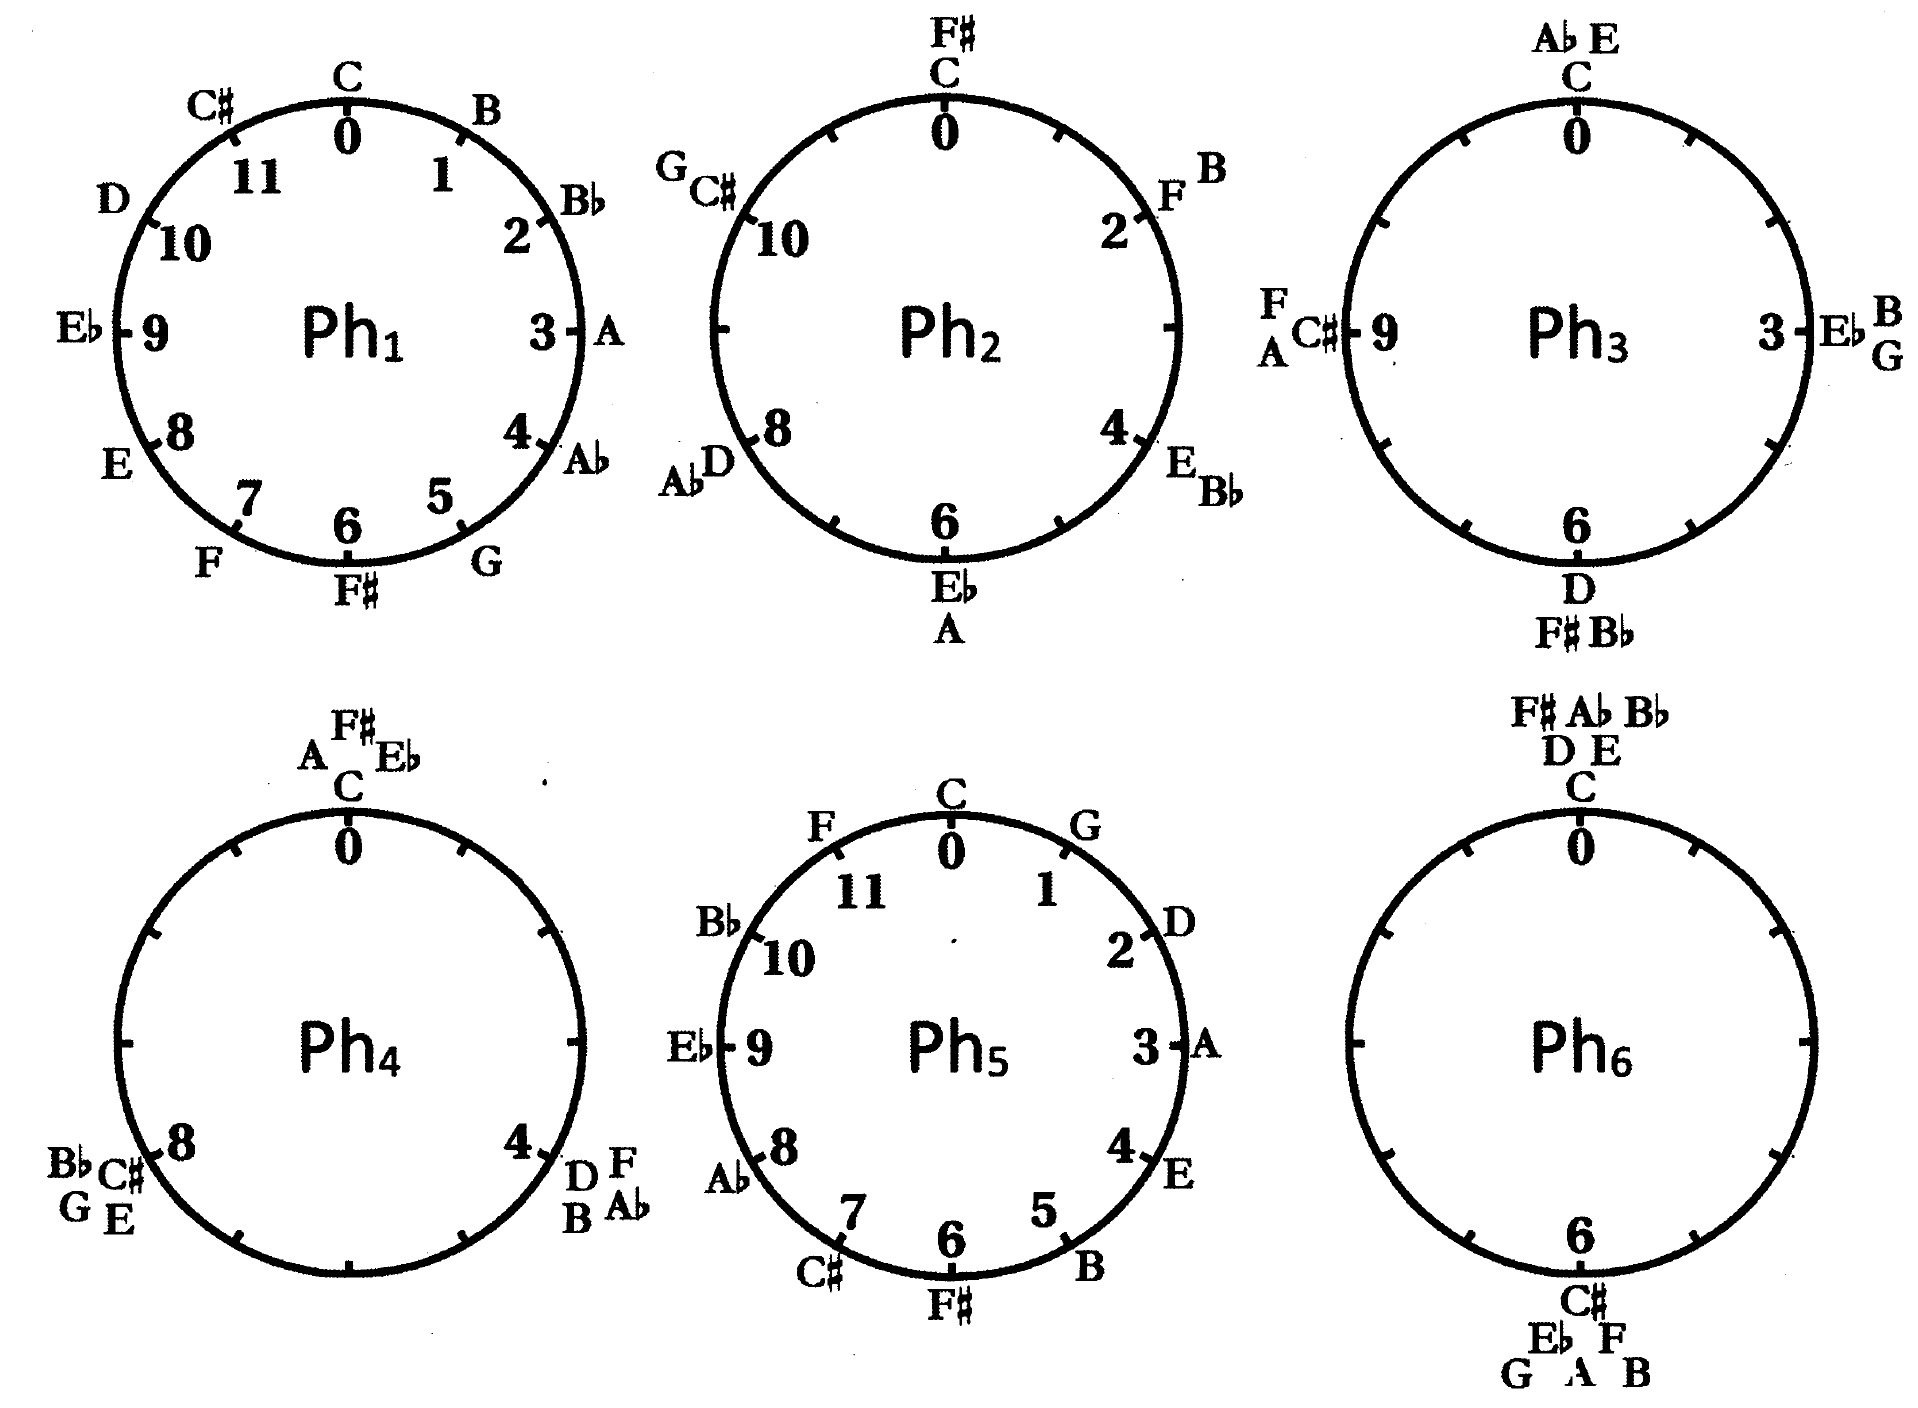
\includegraphics[width=0.5\textwidth]{ph_s.png}
    \caption{Phase Space}
\end{figure}
The process is actually reversible using a more general form of DFT:
\[f_n = \sum_{j=0}^{m} p_i e^{i2\pi jn/m}\frac{1}{m}\], given a full DFT
of a set class by summing up all 12 components, we can find the set class 
by applying the IDFT (inverse DFT process). According to Yust, 
"We can think of the DFT, then, as a way of converting between two 
representations of the same object. One is the raw pitch-class vector, 
which simply tells us how much of each pitch class is present. 
The other, the DFT, represents the pcset (or multiset) as a sum of 
periodic functions." Each component is simply a periodic function of
the phase space. 
\section*{Application}
Another interesting property of the Fourier component is each of them 
represents a typical harmonic quality (scales). According to Yust, "
which we may describe as (1)chromaticism (2) quartal quality, 
(3) hexatonicity, (4) octatonicity, (5) diatonicity, (6) whole-tone."
Since $f_n$ is large when the set class has a small voice leading distance 
to the perfect $n$-note chord, we can use the DFT to apply harmonic analysis
on separate voices. 
\begin{thebibliography}{9}

\bibitem{Temperley}
Temperley, David. "A Bayesian Approach to Key-Finding." In Music and Artificial Intelligence, edited by Christina Anagnostopoulou, Miguel Ferrand, and Alan Smaill, 195–206. Lecture Notes in Computer Science. Berlin, Heidelberg: Springer, 2002.
\bibitem{Tymoczko}
Tymoczko, Dmitri. "Set-Class Similarity, Voice Leading, and the Fourier Transform." Journal of Music Theory 52, no. 2 (2008): 251–72.


\end{thebibliography}
\end{document}
